\documentclass{report}
\usepackage{fontspec}
\usepackage{fancyhdr}
\usepackage{graphicx} % Required for inserting images\
\usepackage[utf8]{inputenc}
\usepackage{lscape}
\usepackage[margin=3cm]{geometry}
\usepackage{listings}
\usepackage[usenames,dvipsnames]{xcolor}
\usepackage{booktabs}
\usepackage{setspace}
\usepackage{comment}
\usepackage{caption}
\usepackage{hyperref}

% for fonts ---------------------------------------------
\setmainfont{Times New Roman}
\setmonofont{JetBrainsMono}[
  Extension=.ttf,
  UprightFont=*-Regular,
  ItalicFont=*-Italic,
  BoldFont=*-Bold,
  BoldItalicFont=*-BoldItalic,
]

%for code styling ---------------------------------------
\definecolor{mBlue}{rgb}{0,0.4,0.7}
\definecolor{mGray}{rgb}{0.5,0.5,0.5}
\definecolor{mPurple}{rgb}{0.58,0,0.82}
\definecolor{backgroundColour}{rgb}{0.92,0.95,0.97}
\definecolor{mAdib}{rgb}{0,0.8,0}
\DeclareCaptionType{code}[Code Snippet][List of Code Listings]

\lstdefinestyle{code}{
    backgroundcolor=\color{backgroundColour},
    commentstyle=\color{mGray},
    keywordstyle=\color{mBlue}\bfseries,
    numberstyle=\color{mGray},
    stringstyle=\color{mPurple},
    basicstyle=\ttfamily\footnotesize,
    breakatwhitespace=false,         
    breaklines=true,                 
    captionpos=b,
    keepspaces=true,                                            
    morekeywords={Input, Output,},
    showspaces=false,                
    showstringspaces=false,
    xleftmargin=5pt,
    %numbers=left,
    numbersep=12pt,
    showtabs=false,                  
    tabsize=4,
    frame=single,
    language=c
}


%Fancy page ---------------------------------------------------
\pagestyle{fancy}
\fancyhf{}

% Variables
\newcommand{\mainTopic}{\huge{Creating Wireframes for Facebook Interface Improvements}}
\newcommand{\mainTopicSmall}{\Large Creating Wireframes for Facebook Interface Improvements}
\newcommand{\coursename}{\Large Software Requirement And Specification}
\newcommand{\coursecode}{\Large SWE 4401}
\newcommand{\reporttype}{\huge{ASSIGNMENT}}

%Fixed Value Variables ----------------------------------------
\newcommand{\Name}{\huge{Khalid Hasan Ador}}
\newcommand{\studentID}{210042102}
\newcommand{\bscProgram}{BSc in Software Engineering}
\newcommand{\dept}{Dept of Computer Science and Engineering}
\newcommand{\university}{\textsc{\Huge{Islamic University of Technology}}}
\newcommand{\univAddress}{Board Bazar, Gazipur, Dhaka, 1704, Bangladesh}

% Header and Footer --------------------------------------------
\fancyhead[L]{\large Assignment}
\fancyhead[R]{\coursename}
\fancyfoot[L]{\large Khalid Hasan Ador (210042102) , BSc in SWE, Dept of CSE, IUT}
\fancyfoot[R]{\large \thepage}

% Header and Footer lines --------------------------------------
\renewcommand{\headrulewidth}{0.4pt} 
\renewcommand{\footrulewidth}{0.4pt}

% Hyperlinks
\hypersetup{
    colorlinks=true,
    linkcolor=black,
    filecolor=magenta,      
    urlcolor=blue,
}

\title{
	\begin{figure}[!htb]
		
\includegraphics[scale=0.2]{IUT.png}
		\centering
	\end{figure}

        \Large{\textbf{\university}}\\	
	\large{\textbf{\univAddress}}\\
    
	\vspace{1.1in}
    \line(1,0){450}\\
        \Large{\textbf{\huge{\mainTopic}}}\\
	\line(1,0){450}\\
	\vspace{0.15in}
	\Large{\textbf{\huge{\reporttype}}}\\
        \vspace{.5in}
	\LARGE{\textbf{\coursecode \ - \coursename}}\\
        \vspace{.2in}
}
\author{
        \Large{\textbf{\Name}}\\\\
        % \vspace{0.1in}
        \Large{\textbf{ID : \studentID}}\\\\
        \Large{\textbf{\bscProgram}}\\\\
        \Large{\textbf{\dept}}
        % \vspace{.2in}
}

\begin{document}

\maketitle
\large
\tableofcontents


\chapter{\mainTopic}

\section{LogIn Page}
\subsection{Concept-1}

\textbf{Concept:} Wireframe an inviting and secure entry point. 

\begin{figure}[h]
    \centering
    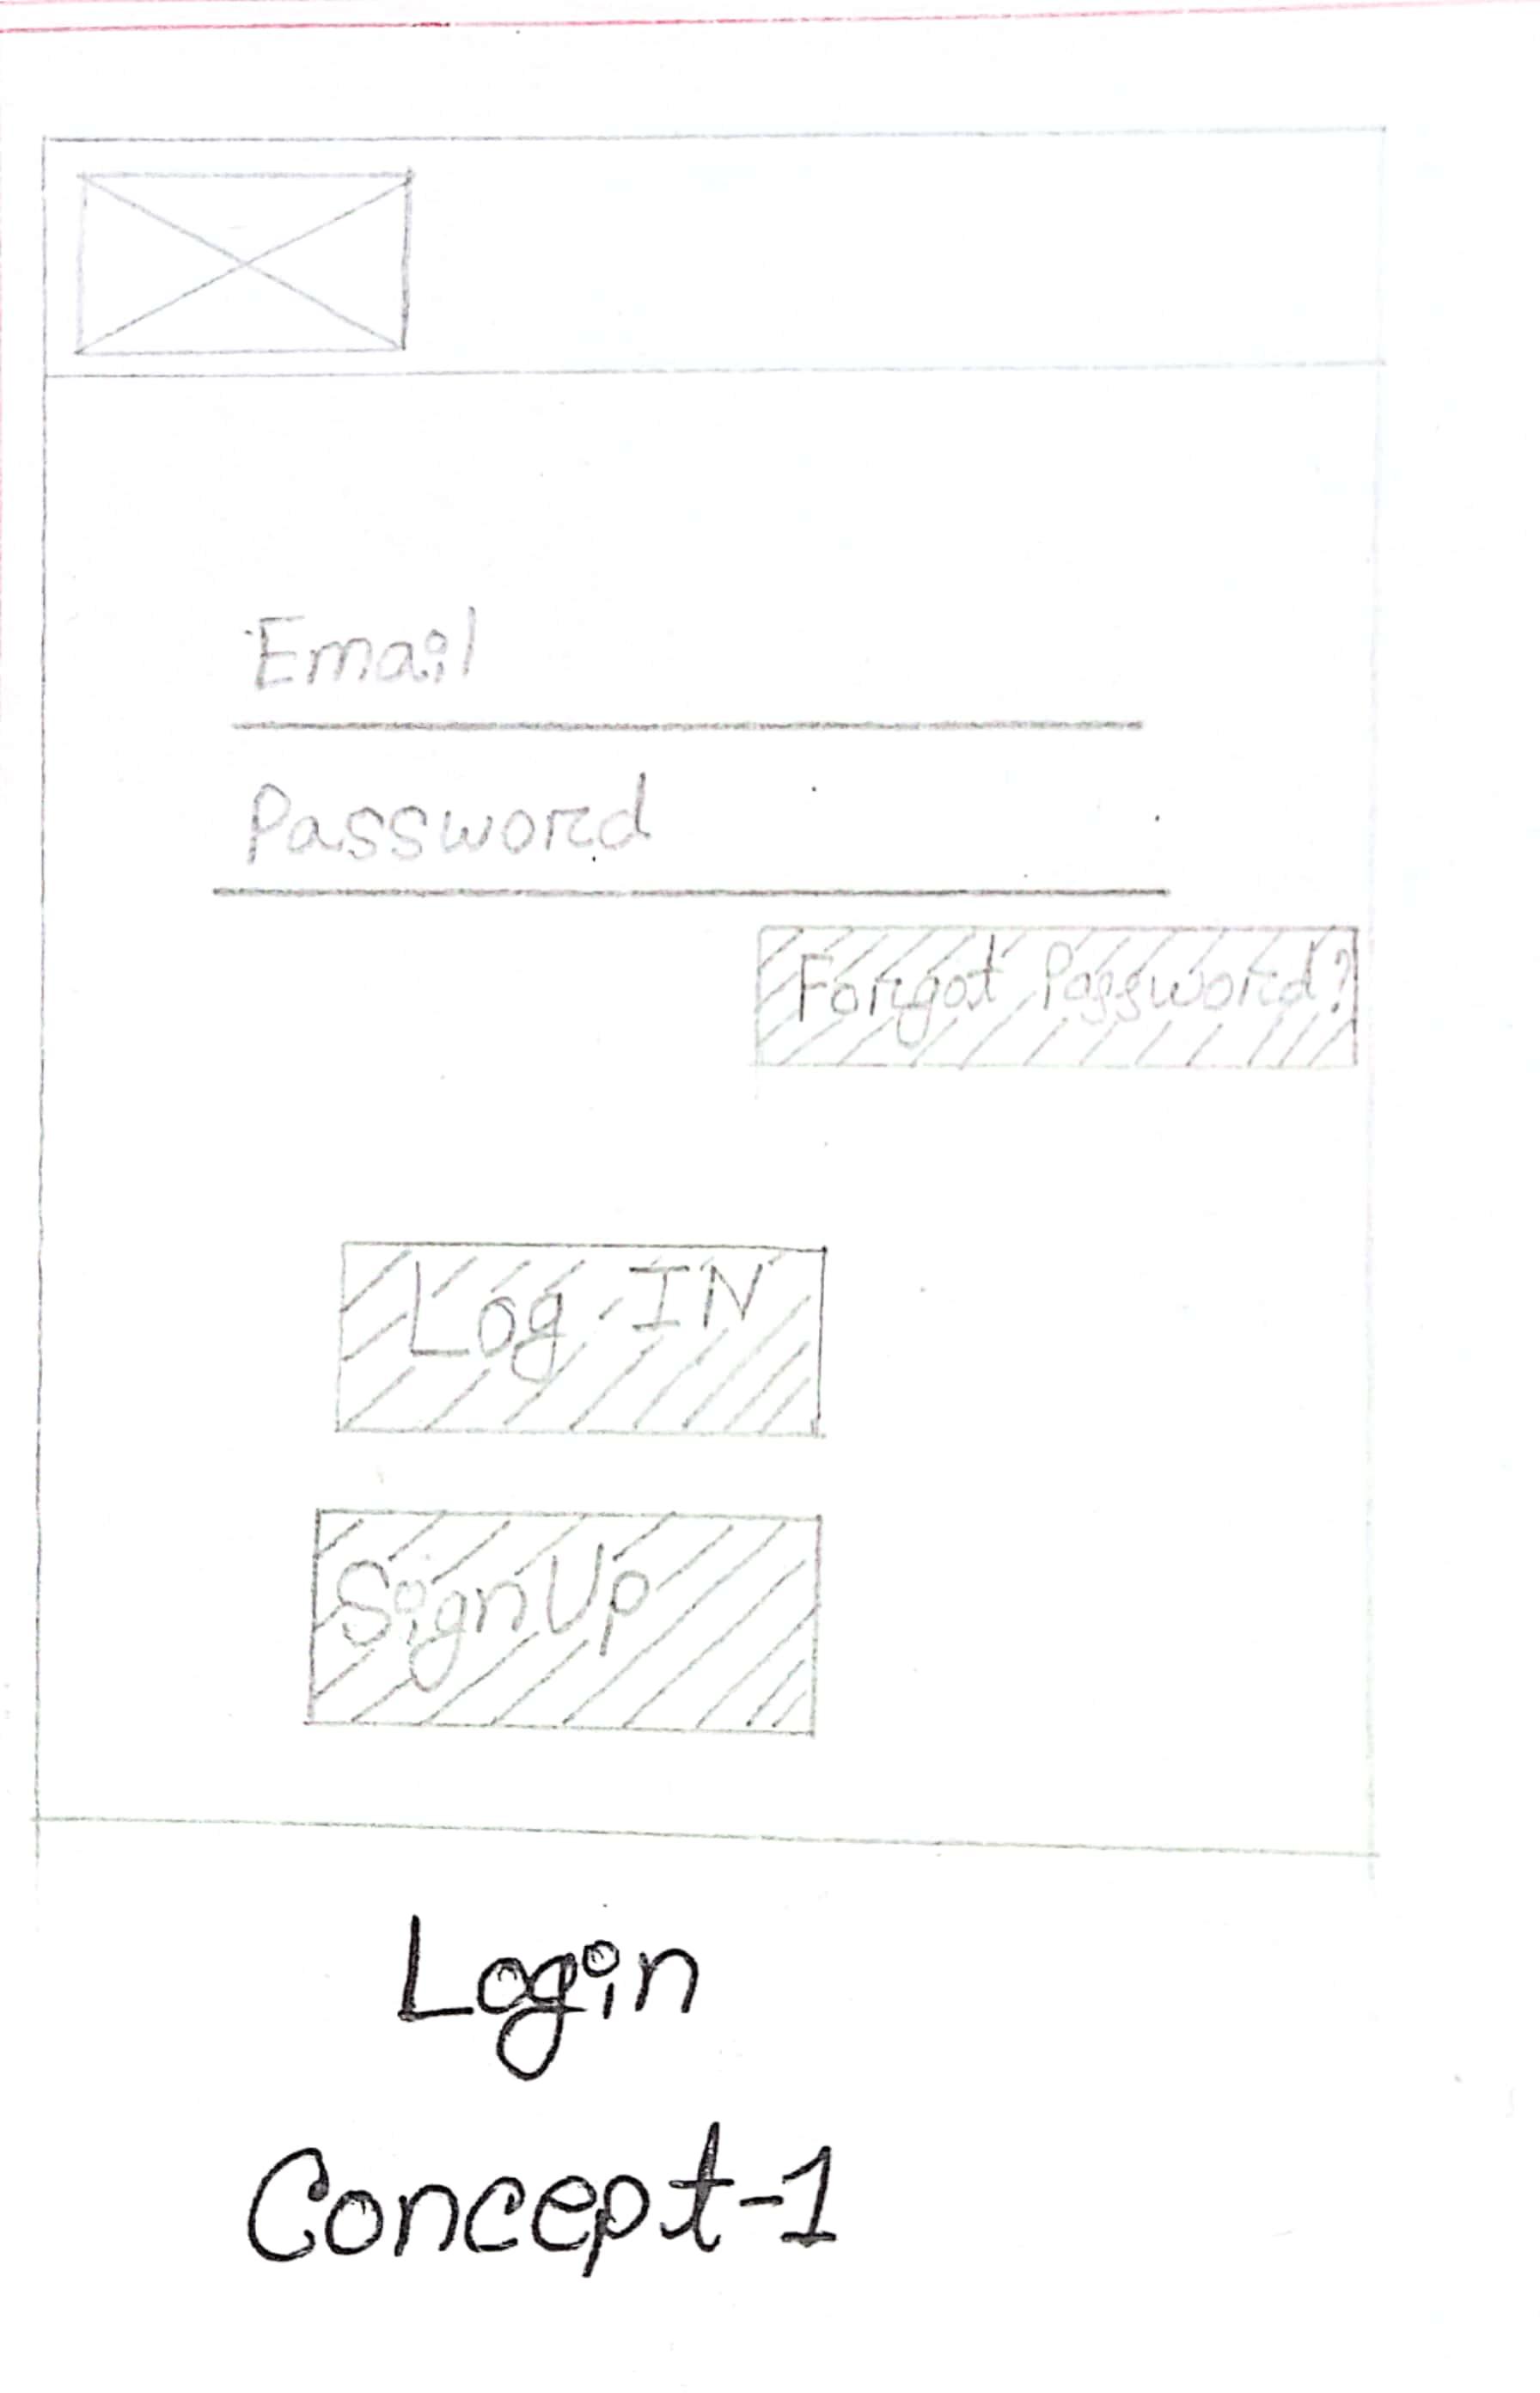
\includegraphics[width=0.5\linewidth]{1.jpg}
    \label{fig:enter-label}
\end{figure}

\textbf{Description:} The idea was to create an inviting and secure entry point. The above login wireframe is very simple and secure as you will always need a password to login. Besides it works fine a a login page. We have the option to Enter E-mail and password to login. If we somehow forget our password, we have the forget password button. For users who don't have an account yet, we have the SignUp button.


\subsection{Concept-2}
\textbf{Concept-2: }Create a wireframe that integrates advanced security features seamlessly.

\begin{figure}[h]
    \centering
    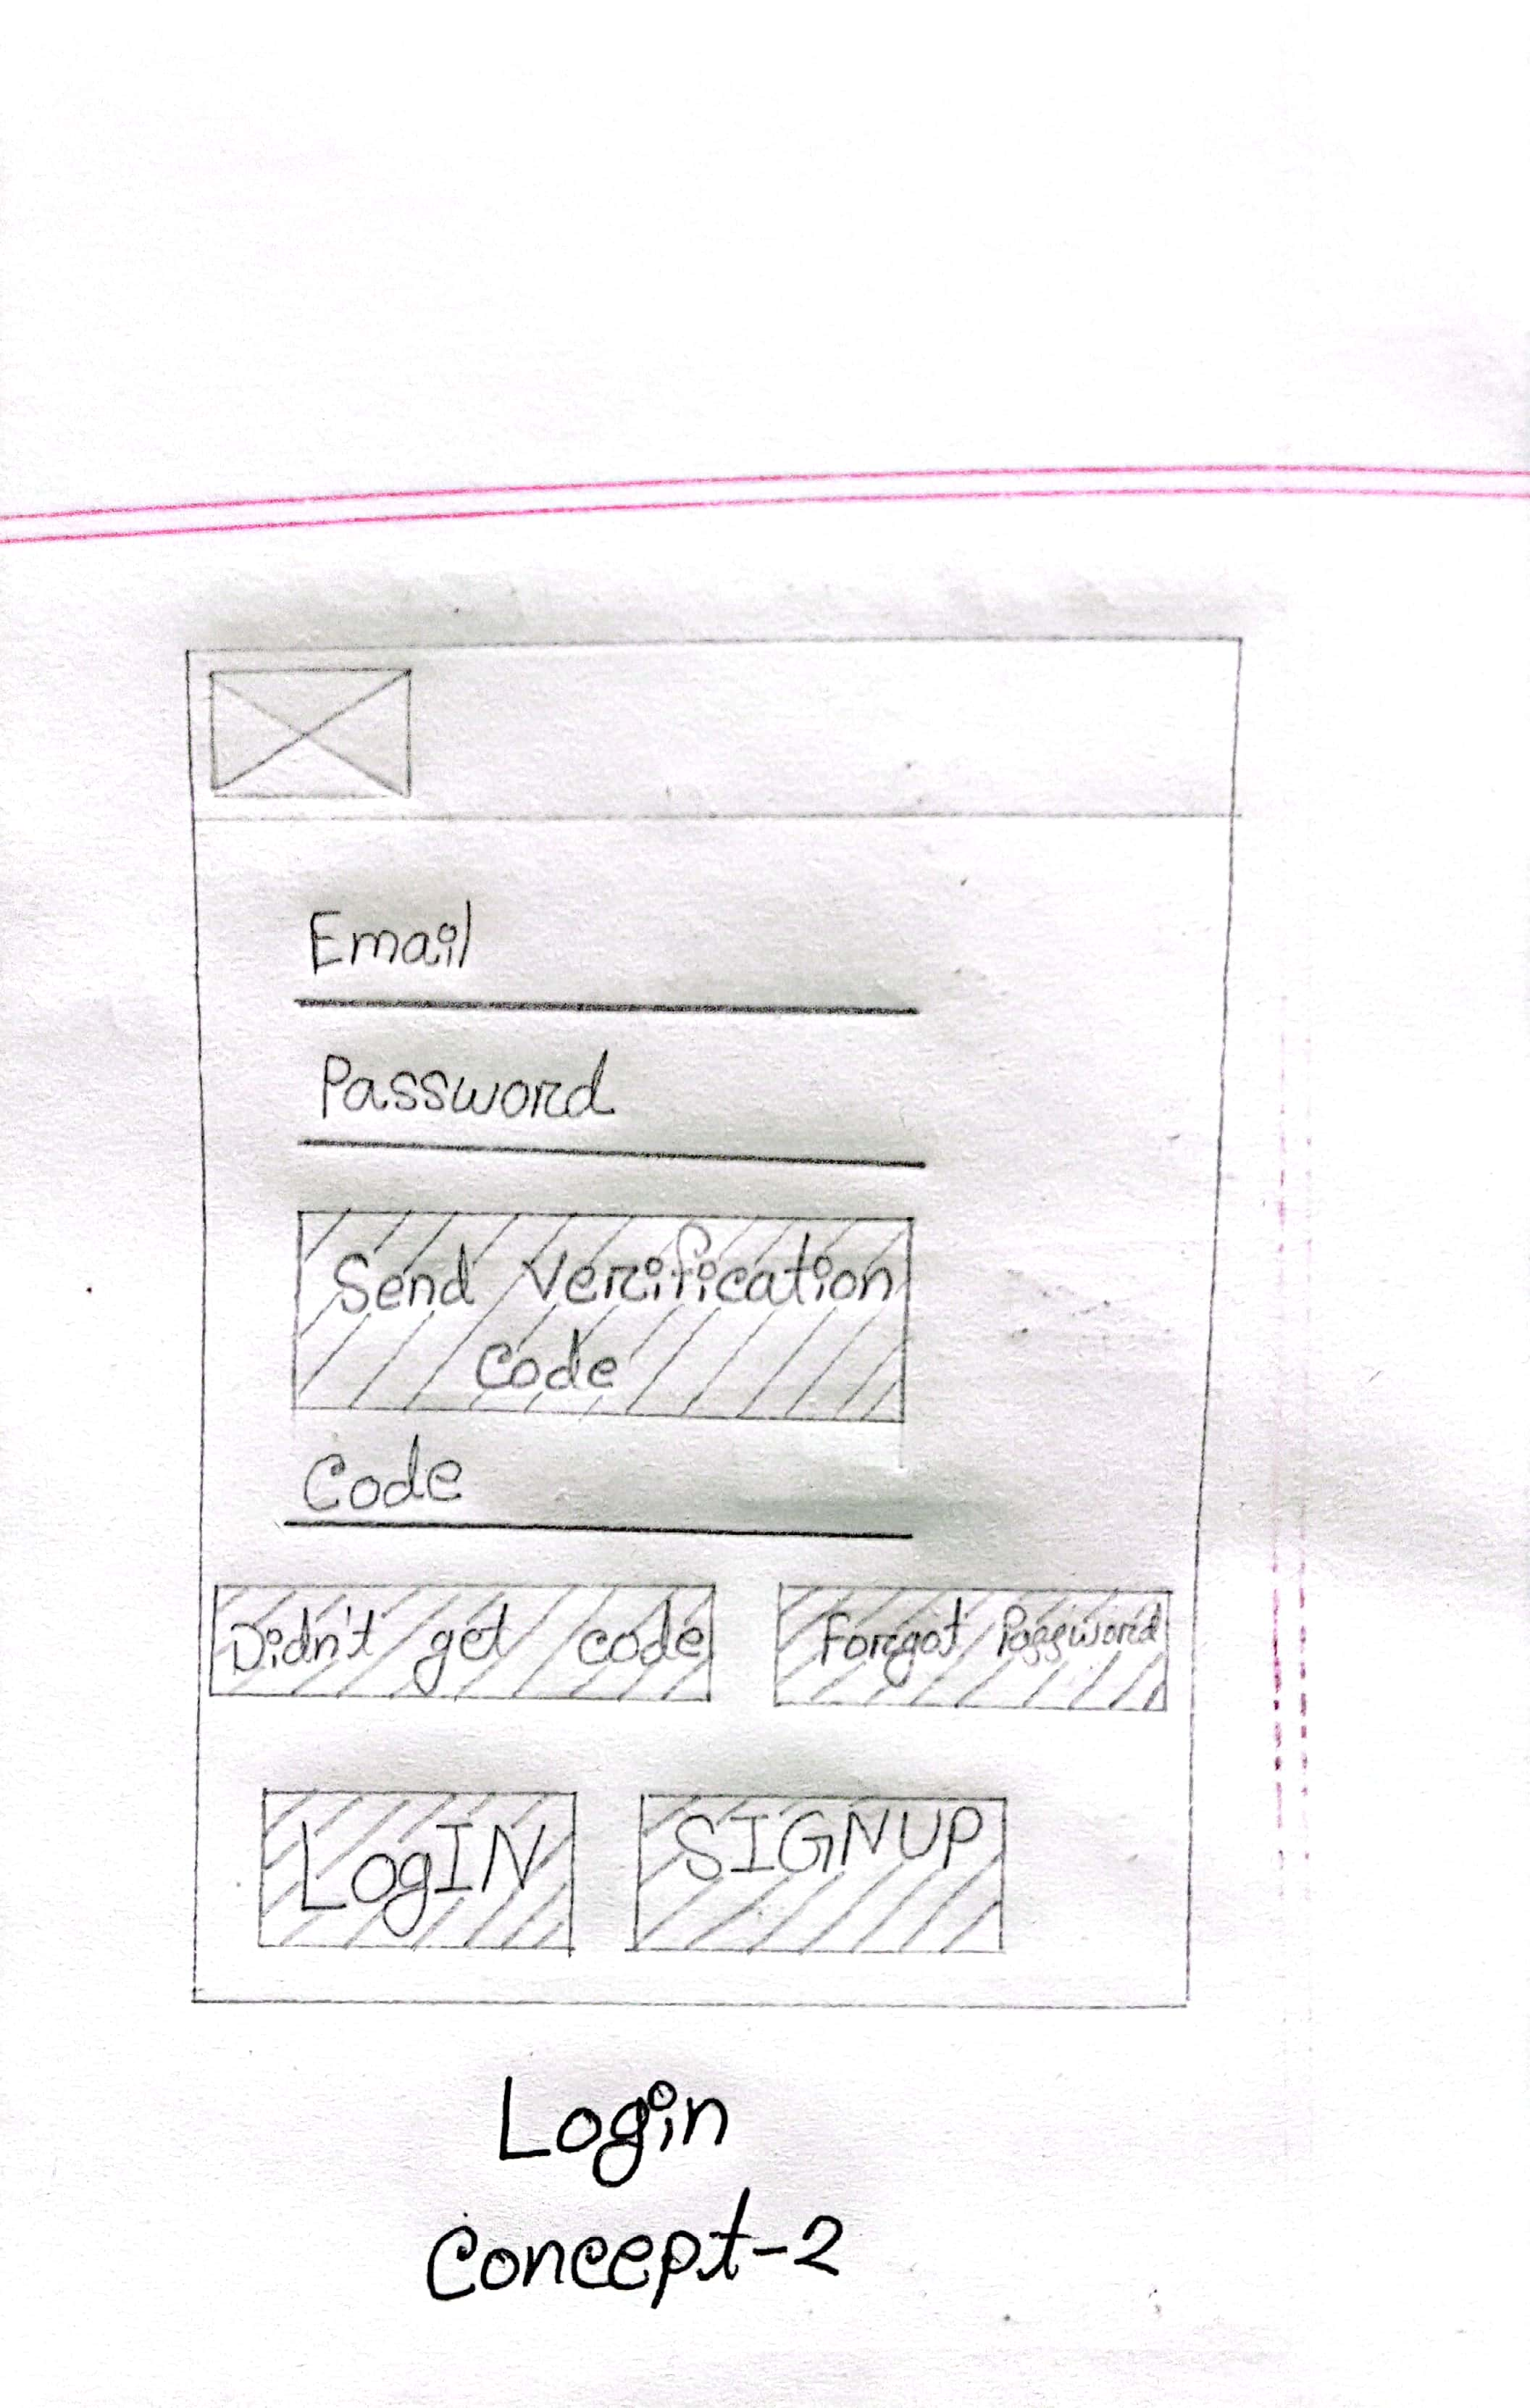
\includegraphics[width=0.5\linewidth]{2.jpg}
    %%\caption{Enter Caption}
    \label{fig:enter-label}
\end{figure}


\textbf{Description: } Here we needed to integrate advanced security feature. So i added an option for verification. After filling the E-mail and PassWord section users can click on the button "Send Verification Code". It will send a code in their mail and they will need that One-Time-Code to login to their account. Additionally we have a "Didn't get code" button in case users does not receive the code for some reasons.


\newpage



\section{Newsfeed}
\subsection{Concept-1}
\textbf{Concept: }Wireframe a version that boosts how users discover and interact with content.

\begin{figure}[h]
    \centering
    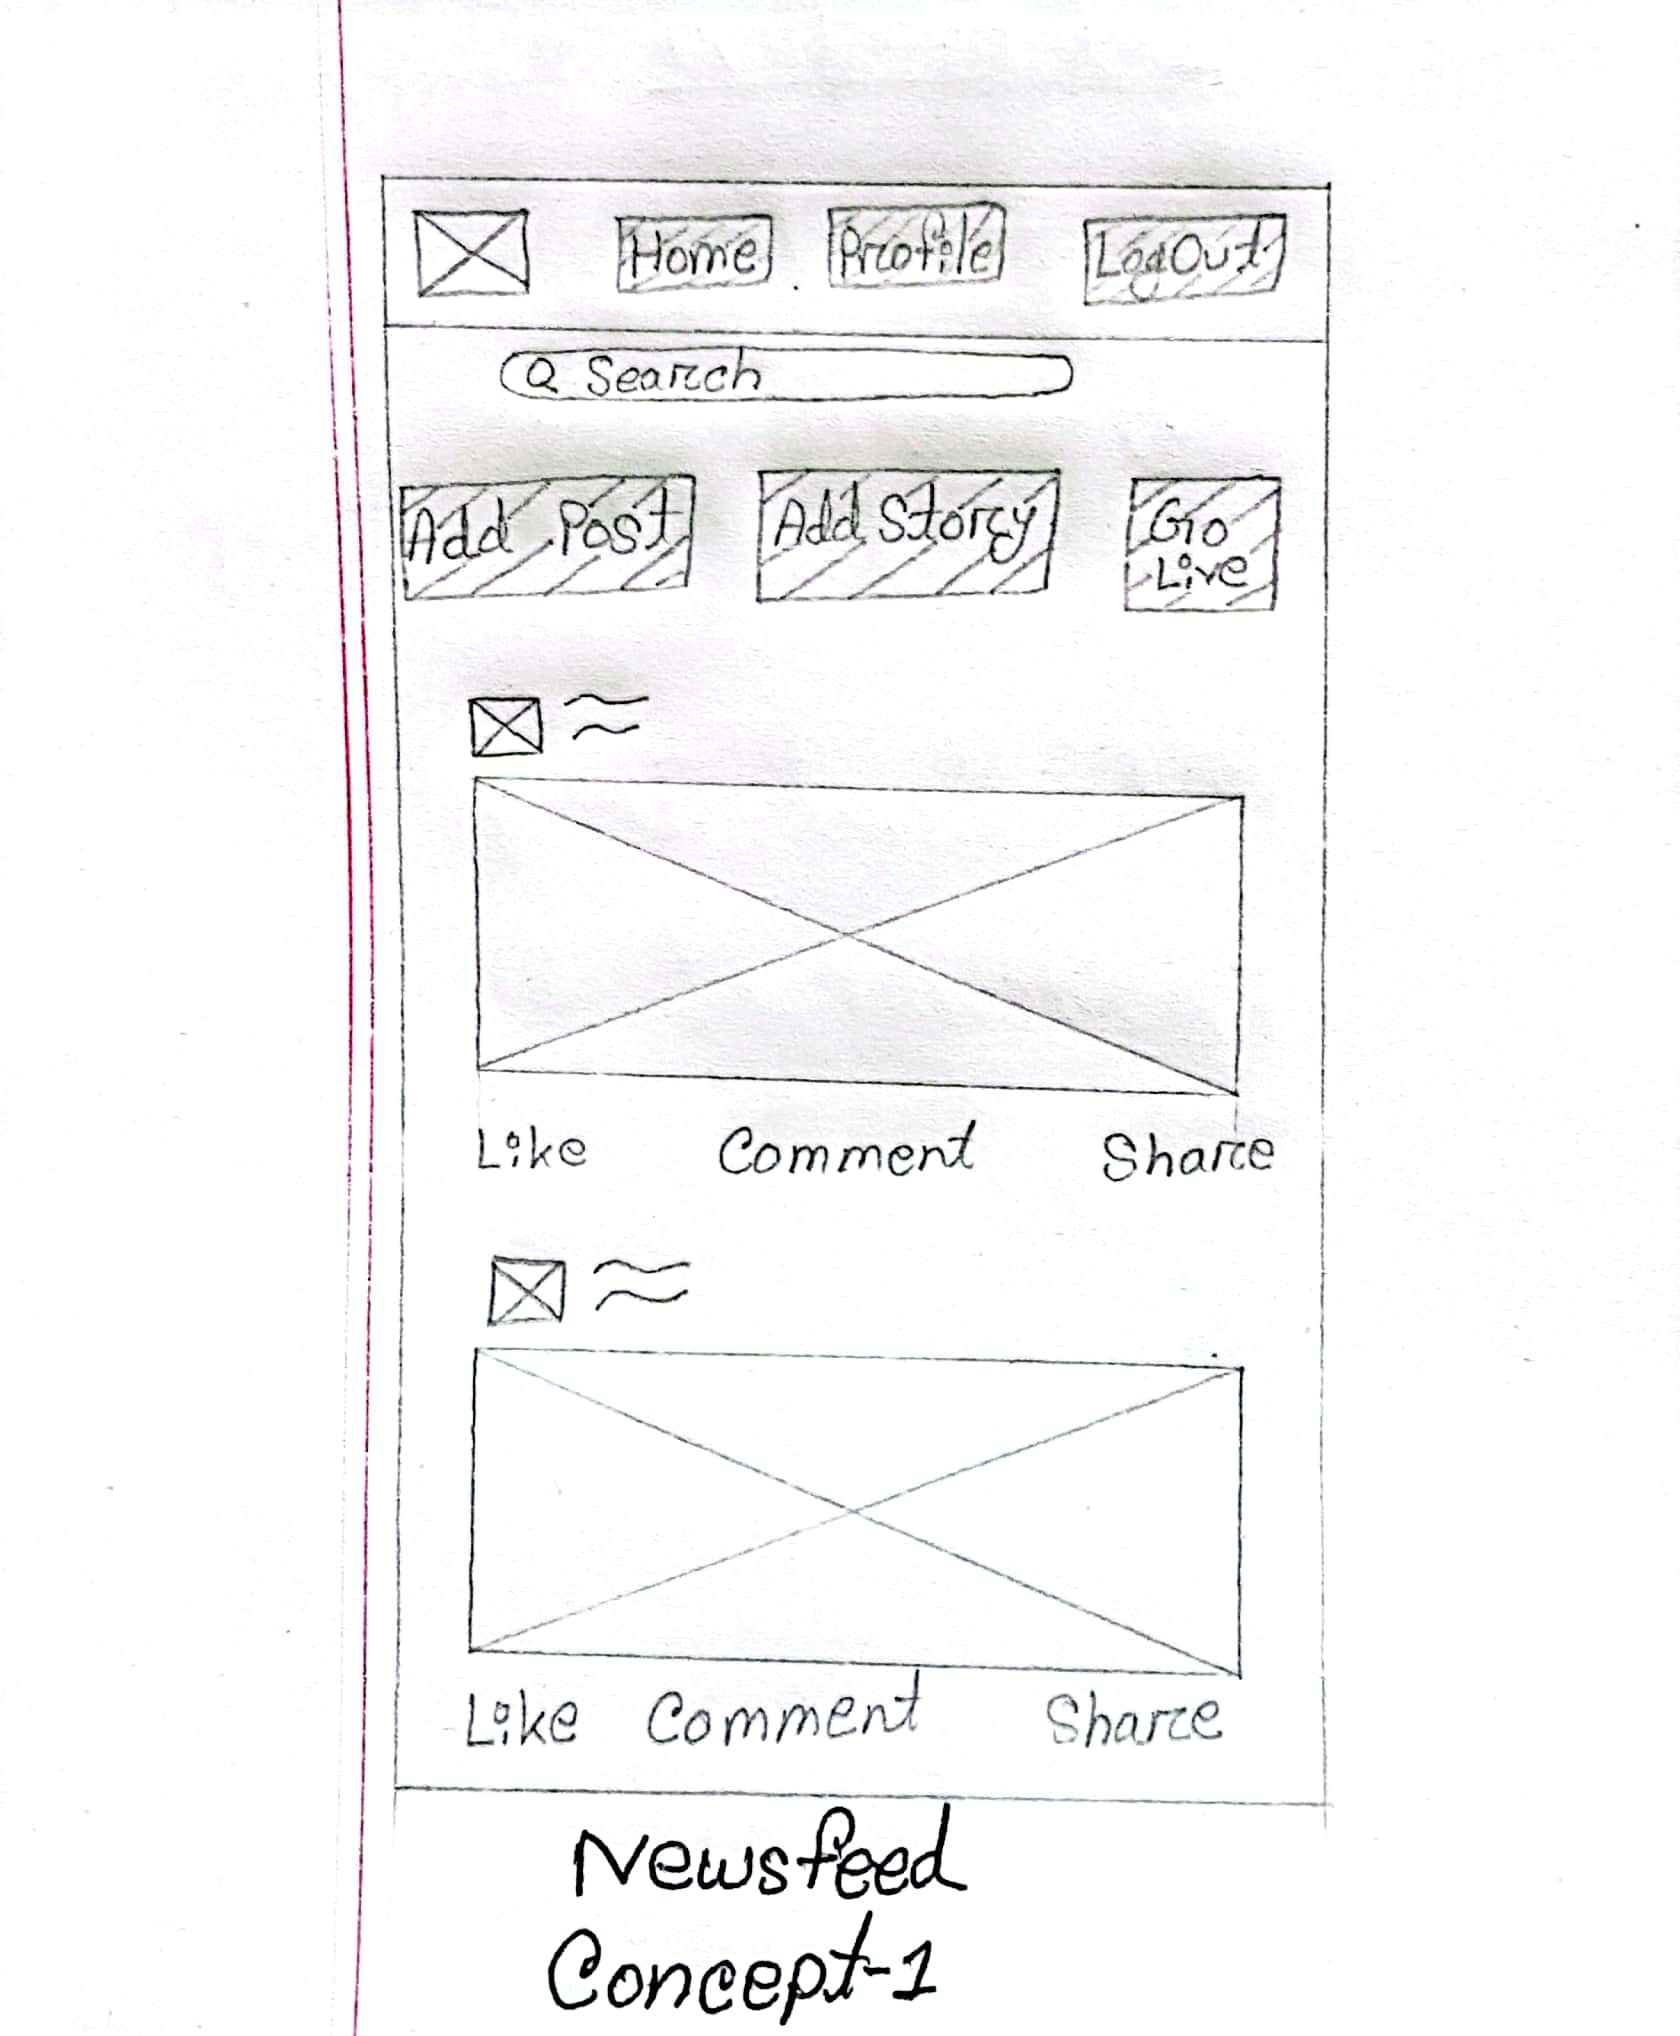
\includegraphics[width=0.5\linewidth]{3.jpg}
    %%\caption{Enter Caption}
    \label{fig:enter-label}
\end{figure}

\textbf{Description: }The job was to make it easier for users to discover and interact with contents. So we have all the contents listed one after another at random to make it easier for the user to interact. At the beginning we have a search bar. So that users can easily search anything they are looking for. Besides, we have buttons like "Add Post", "Add Story" and "Go Live" at the top for user convenience. "Add Post" will help users to add new post. "Add Story" will help users to add new story. With every content at the top the user who posted that is mentioned and at the bottom there are option to "Like", "Comment" and "Share".



\newpage



\subsection{Concept-2}
\textbf{Concept: }Develop a wireframe that emphasizes a streamlined content presentation.

\begin{figure}[htb]
    \centering
    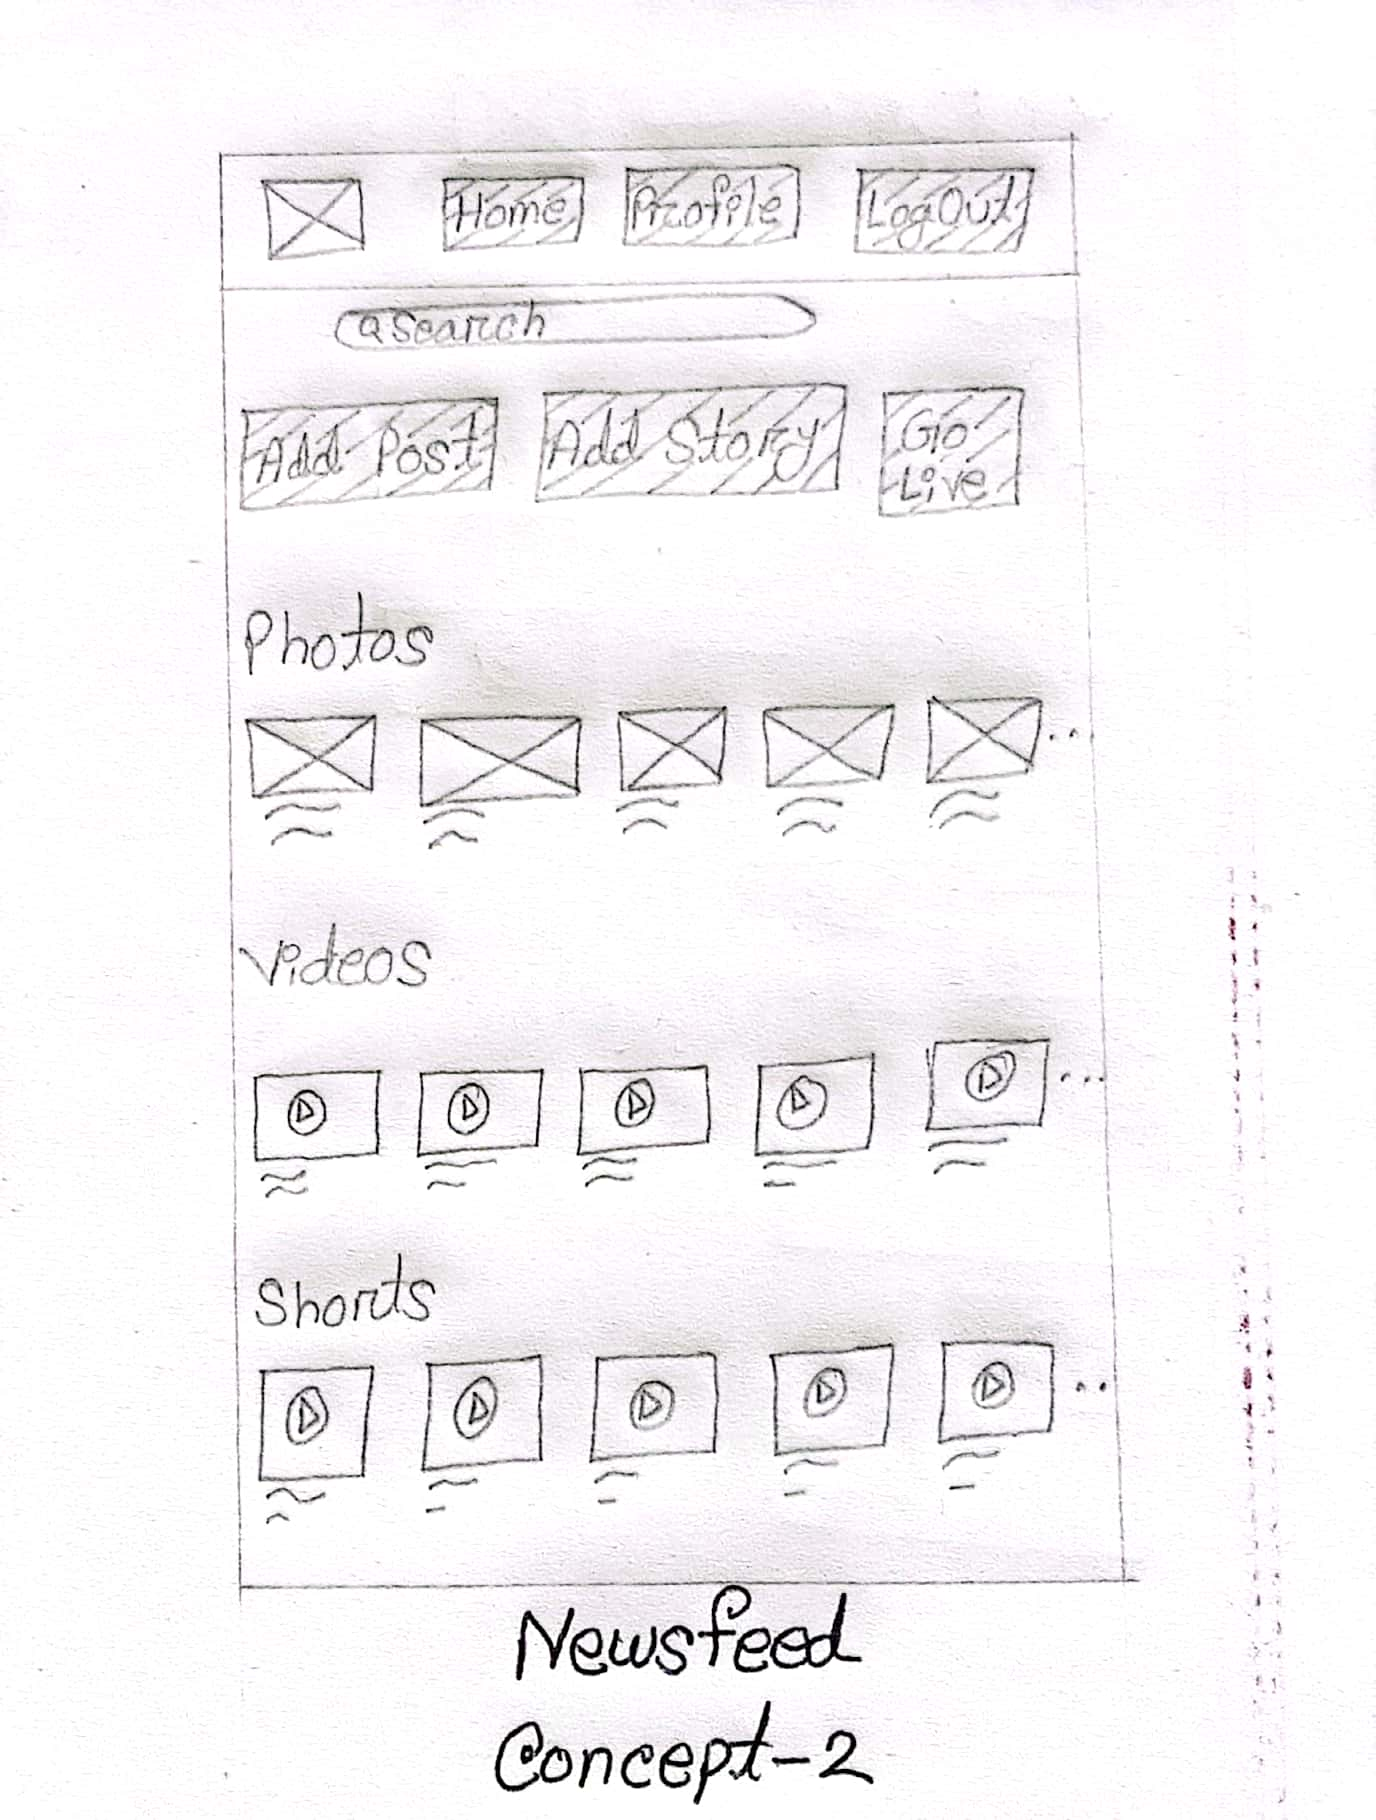
\includegraphics[width=0.5\linewidth]{4.jpg}
    %%\caption{Enter Caption}
    \label{fig:enter-label}
\end{figure}

\textbf{Description: }The job was to make a streamlined content presentation. So in this wireframe we made different sections for each kind of content. In the Photos Section, photos posted by my friends will show up. We can slide to the right to see more photos. They can do the same for videos and Shorts. Besides, we have buttons like "Add Post", "Add Story" and "Go Live" at the top for user convenience. "Add Post" will help users to add new post. "Add Story" will help users to add new story. With every content at the top the user who posted that is mentioned and at the bottom there are option to "Like", "Comment" and "Share".







\newpage




\section{Profile Page}

\subsection{Concept-1}
\textbf{Concept: }Produce a wireframe showcasing enhanced personalization and activity highlights.

\begin{figure}[h]
    \centering
    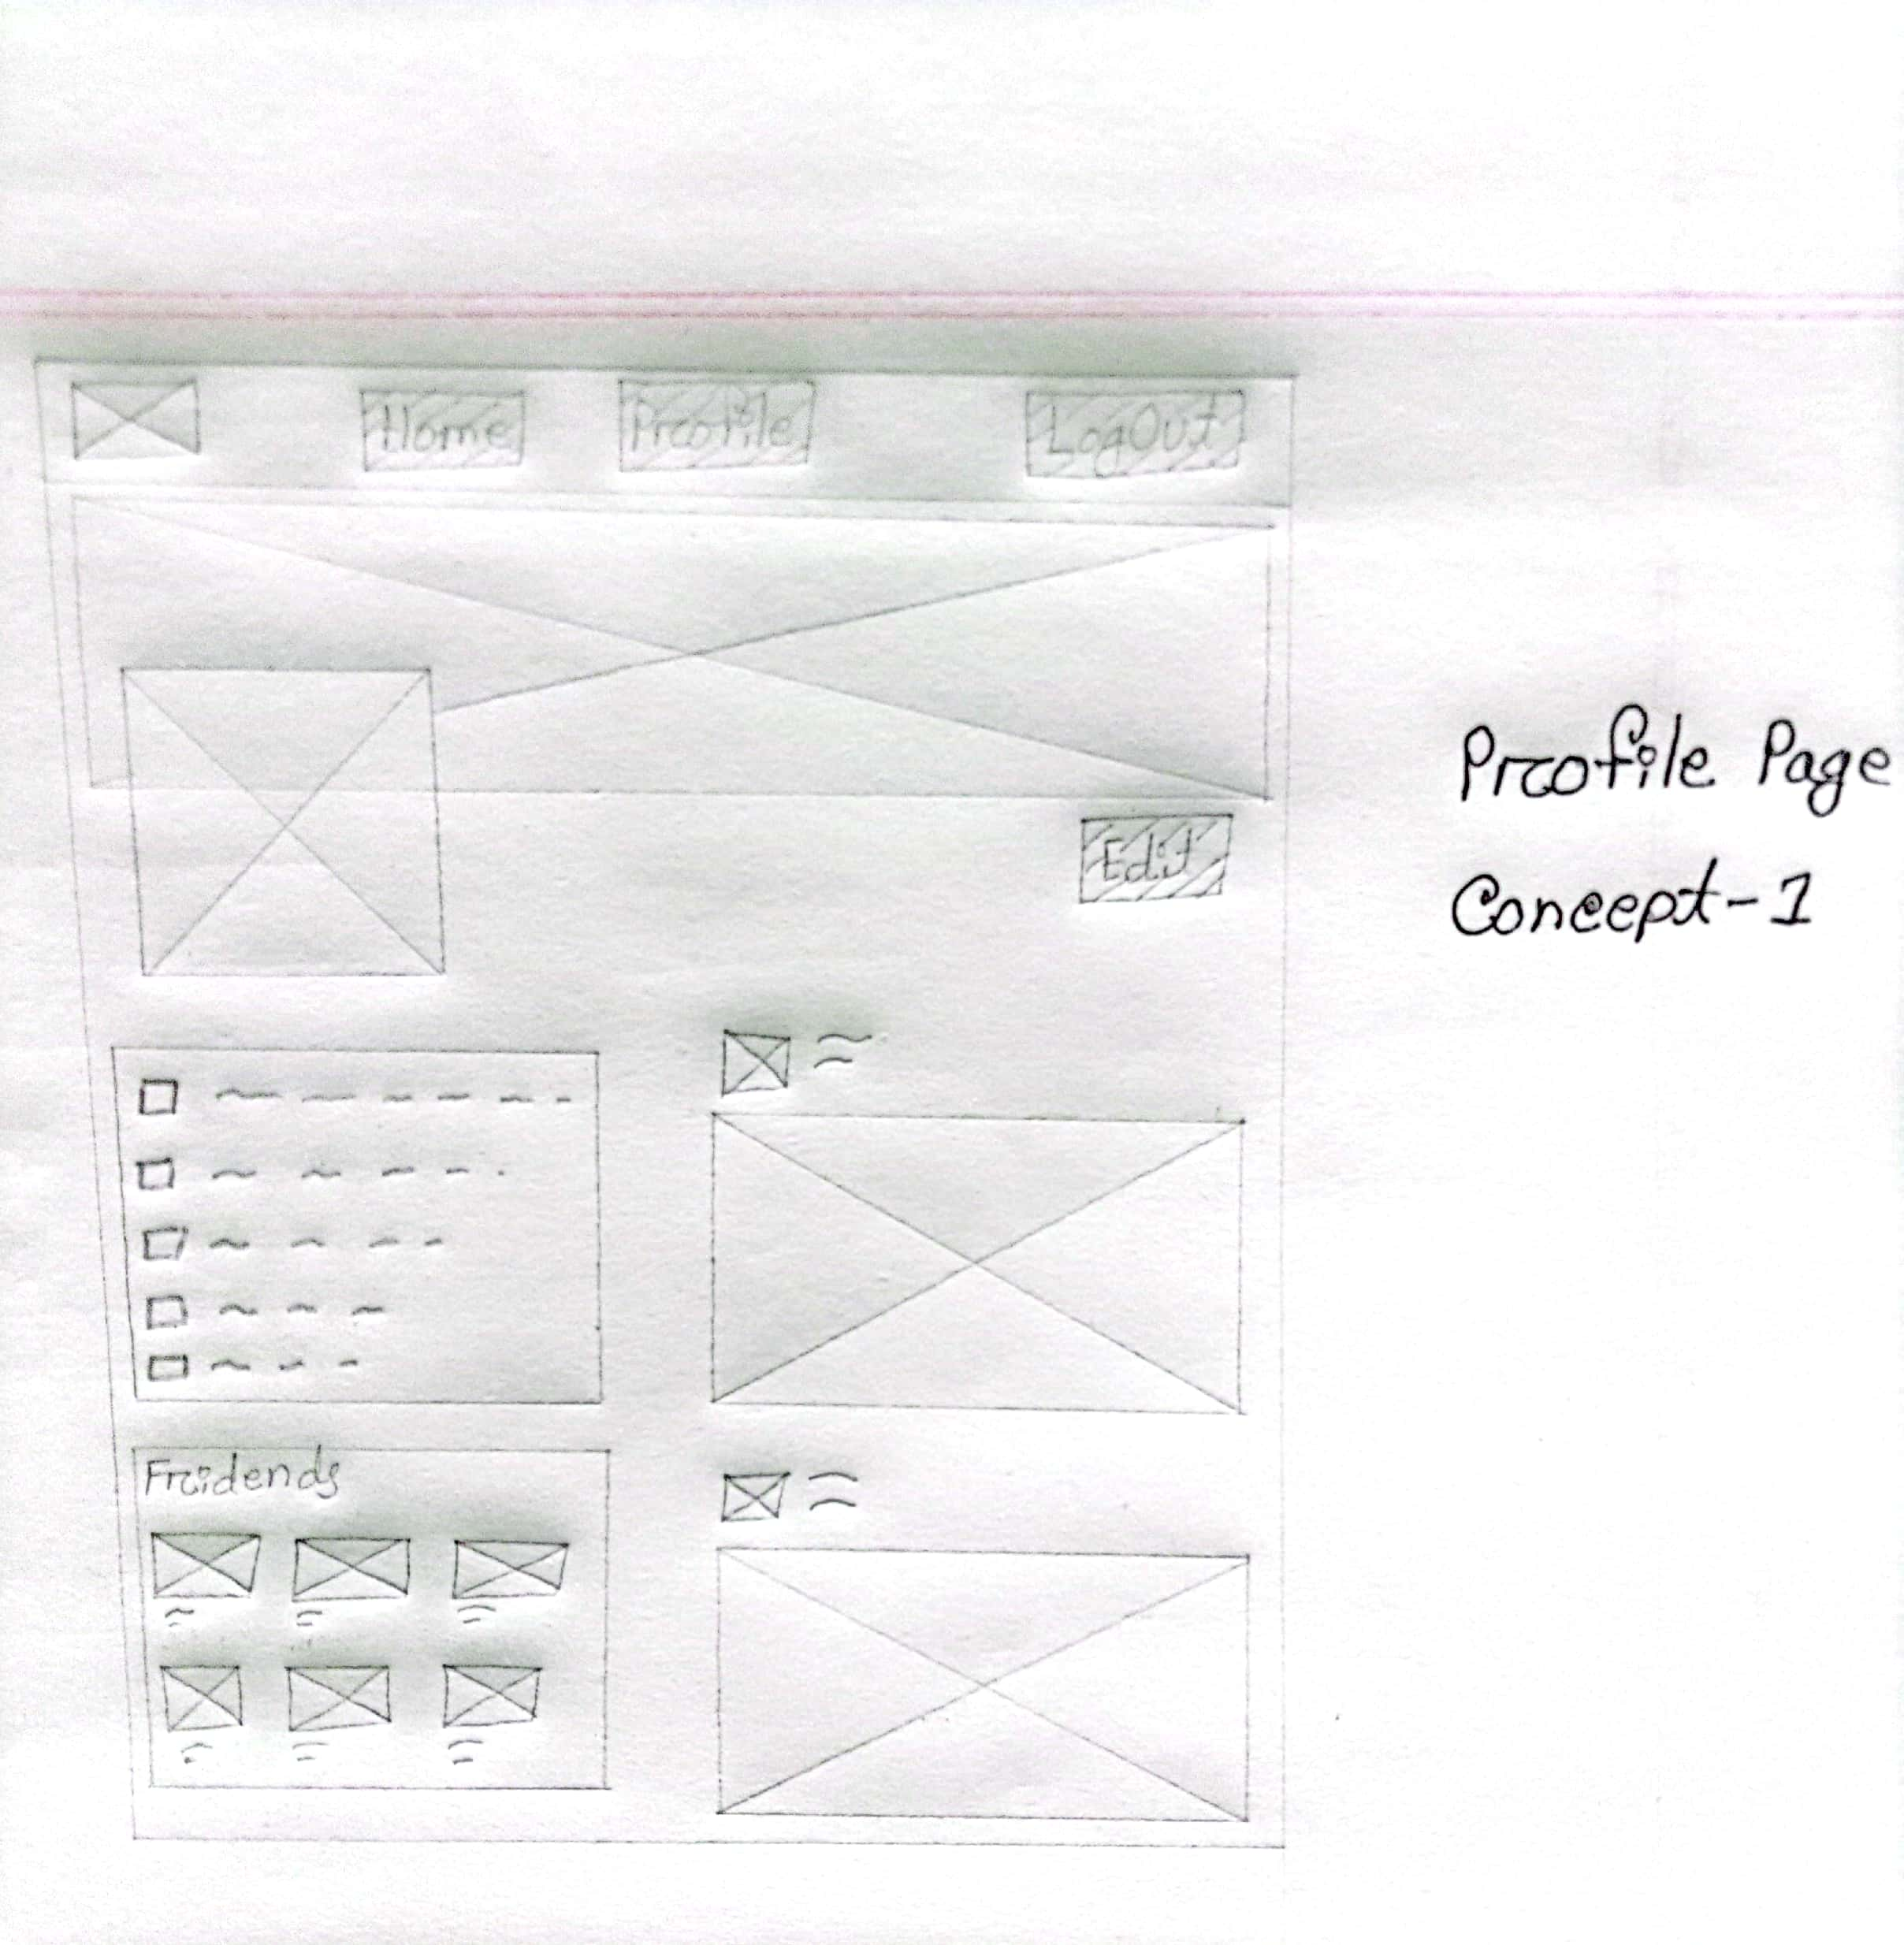
\includegraphics[width=0.5\linewidth]{5.jpg}
    %%\caption{Enter Caption}
    \label{fig:enter-label}
\end{figure}


\textbf{Description: }The focus was on personalization and activity highlights. The wireframe of the Profile Page has a Profile Picture and a Cover Photo. Then we have the "Edit" button so that users can personalize their profile according to their will. Then at the left side we have 2 sections. 1 for info of the user namely INTRO Section and other section shows some friends of the user.\\

And at the left side we have listed all the contents posted by the user himself. This is the activity section where users can review their activities.


\newpage



\subsection{Concept-2}

\textbf{Concept: }Create a wireframe focused on simplified navigation and content interaction.

\begin{figure}[h]
    \centering
    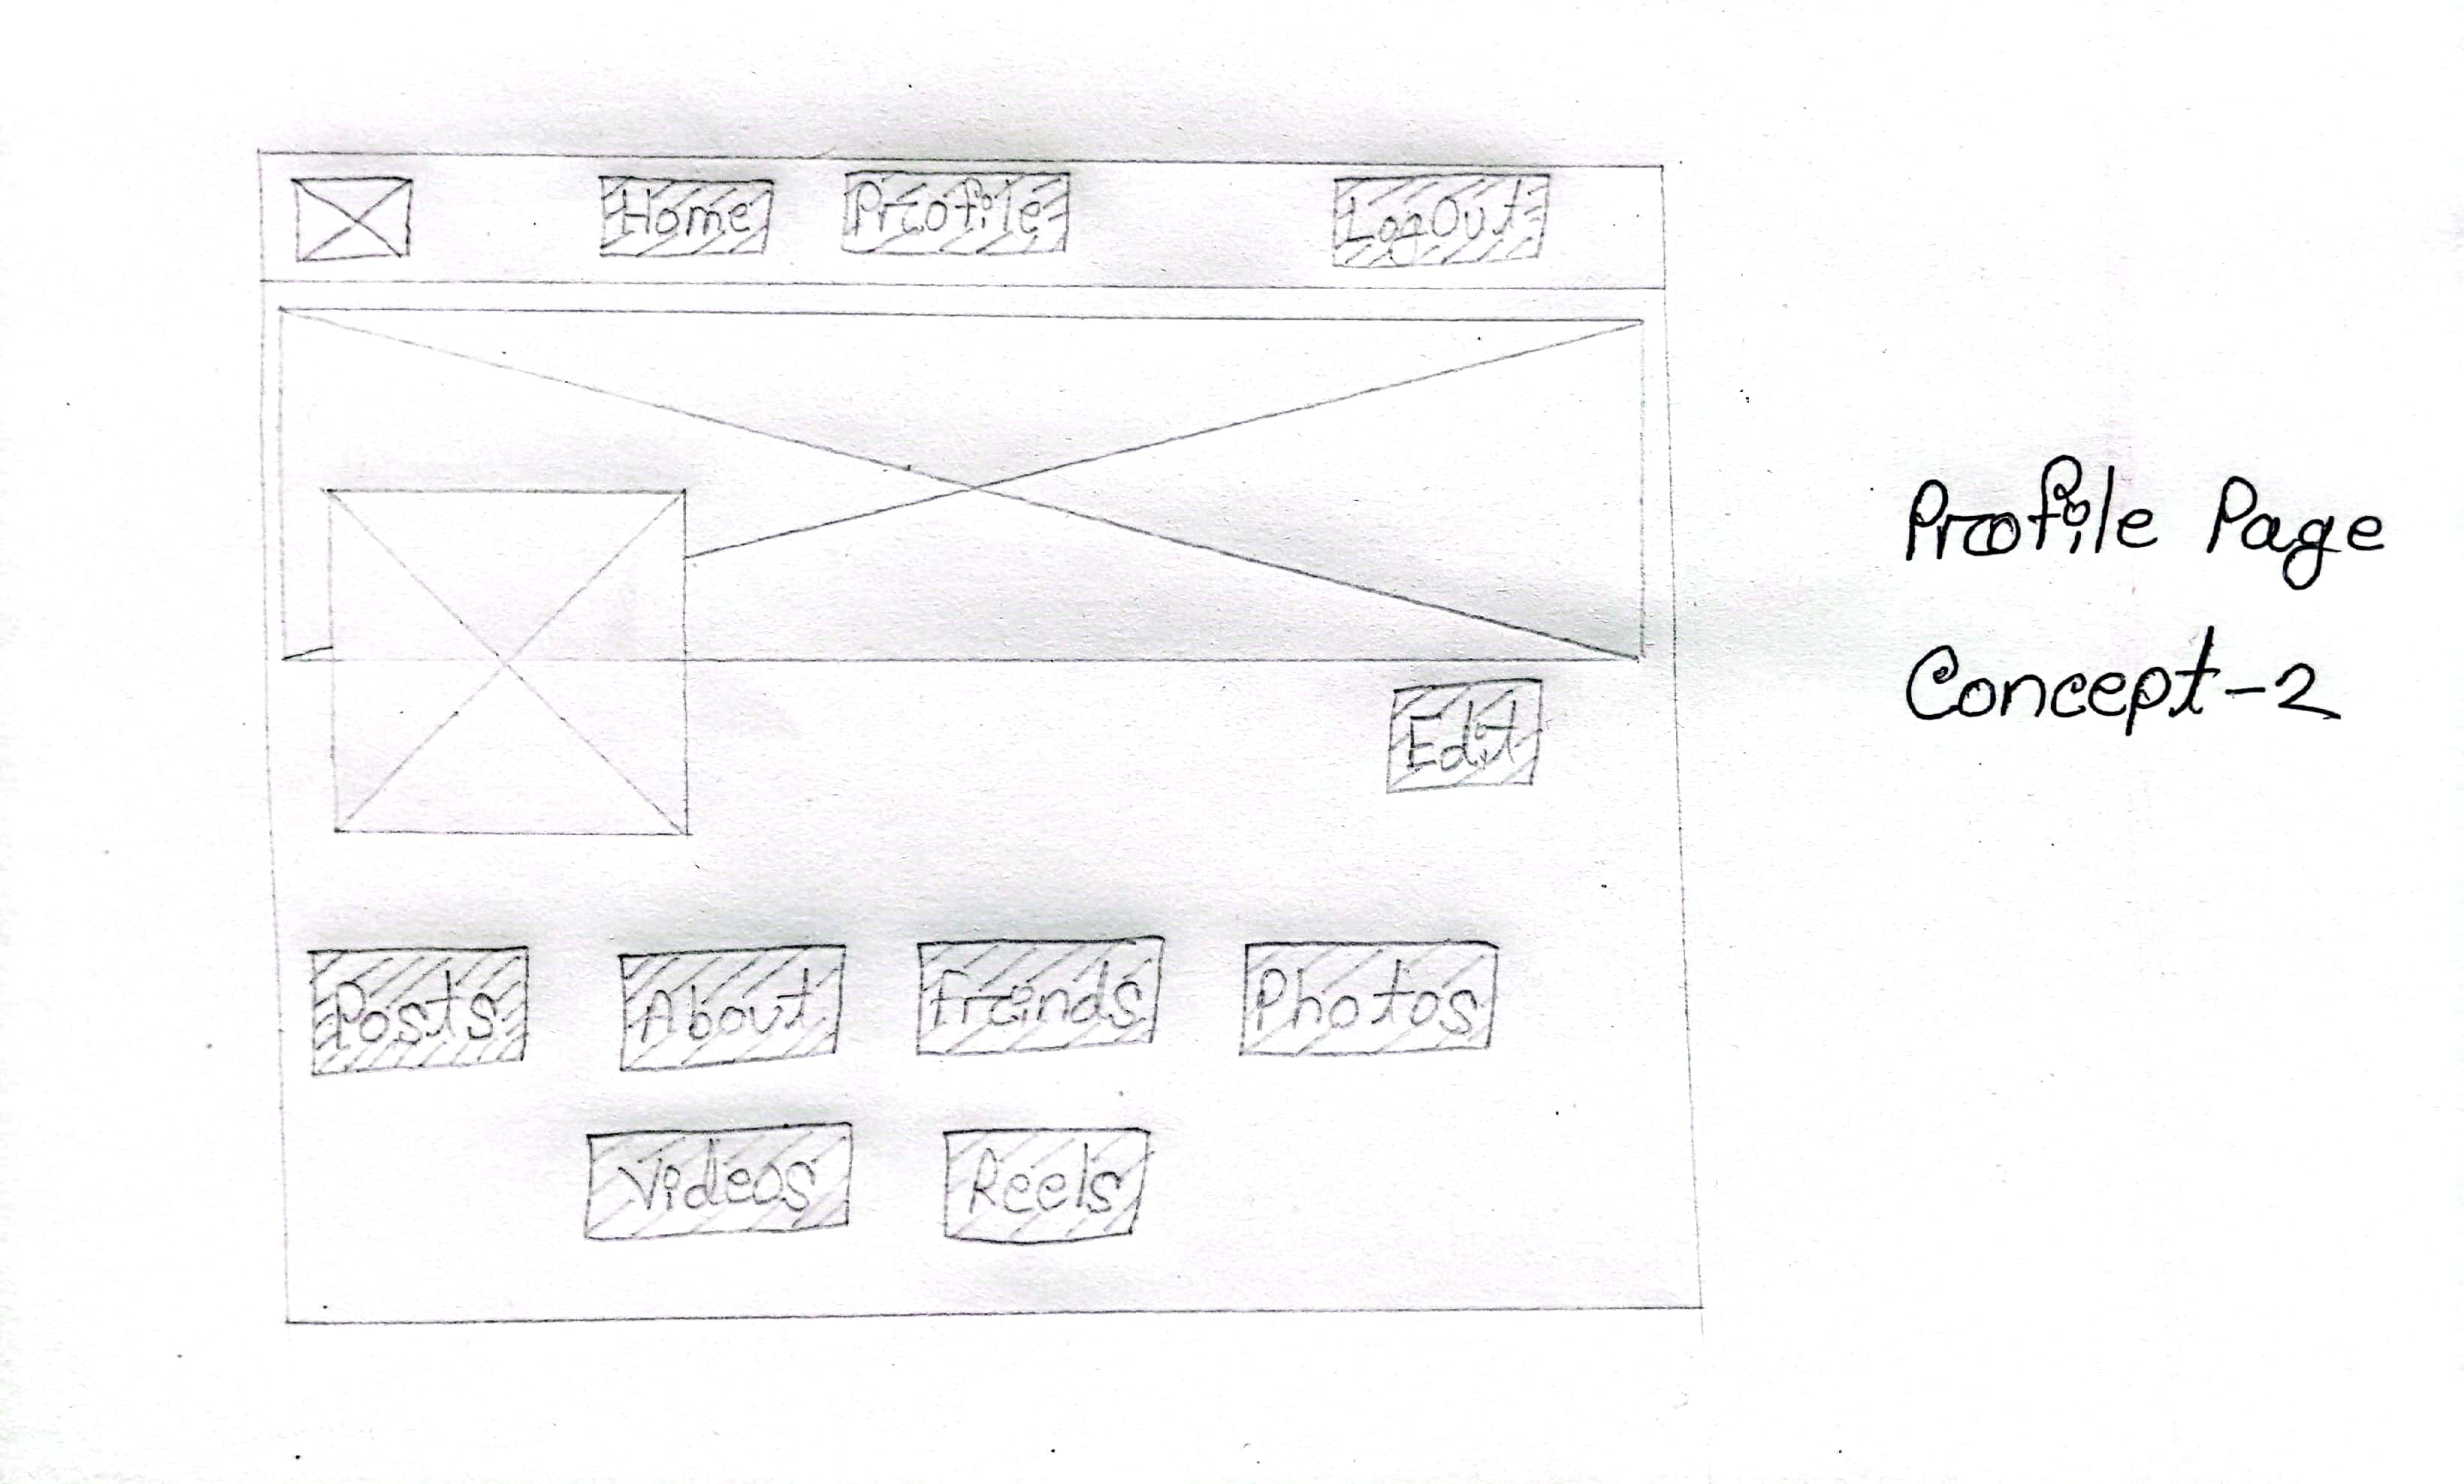
\includegraphics[width=0.5\linewidth]{6.jpg}
    %%\caption{Enter Caption}
    \label{fig:enter-label}
\end{figure}


\textbf{Description: }We had to create a simplified navigation system for the user. So instead of having everything in one single page in this wireframe we just have the buttons to navigate through everything.
\begin{enumerate}
    \item \textbf{Posts: }To see previous posts.
    \item \textbf{About: }To see user info.
    \item \textbf{Friends: }To see the list of friends.
    \item \textbf{Photos: }To see the photos user posted.
    \item \textbf{Videos: }To see the videos user posted.
    \item \textbf{Reels: }To see the shorts user posted.
\end{enumerate}


\end{document}
